% Section 1 of manuscript v0.2 (docs/paper/manuscript.md), converted without changes to claims or numbers.
\section{Introduction}\label{sec:intro}

\subsection{What the operator needs to see}\label{sec:intro-need}

Industrial sucrose production runs as a sequence of evaporative-cooling crystallization ``strikes'' in vacuum pans. A
typical white-sugar plant operates a three-massecuite scheme --- A-, B-, and C-product --- each of which is charged
with purified syrup, concentrated to the meta-stable supersaturated state, \textbf{seeded} with a small mass of milled
sugar or magma, and then run for \textbf{three to four hours} while supersaturation is held in the growth region by
controlled vapour-pressure decrease \citep{Bubnik1995,Asadi2006}. Throughout the strike, the operator must intervene
with sweetwater additions, vacuum and temperature setpoints, and timing of cuts and discharges. The two parameters
that ultimately matter to the plant are the \textbf{mean aperture (MA)} and the \textbf{coefficient of variation (CV)}
of the discharged crystal-size distribution: MA drives downstream classification, CV controls centrifuge efficiency
and the recoverable molasses fraction. A strike that lands on the wrong MA or with excessive CV must be reworked at
substantial energy and yield cost.

Without a calibrated, real-time view of the in-vessel CSD, operator interventions rely on indirect proxies ---
conductivity, refractive index, boiling-point elevation --- that are coupled to CSD only through plant-specific
heuristics. \textbf{A reliable, non-invasive, in-line crystal-size measurement is among the most-requested unsolved
sensor problems in industrial crystallization} \citep{Nagy2013,Simon2015}.

\subsection{Why the dominant instruments fall short}\label{sec:intro-instruments}

Four families of measurement principle dominate the literature on in-line CSD monitoring; each has well-documented
limitations.

\paragraph{Probe-based optical instruments} Mettler-Toledo's \emph{Focused Beam Reflectance Measurement} (FBRM) scans
a laser through the slurry and infers a chord-length distribution from back-scattered pulses
\citep{Worlitschek2003,Heath2002}. FBRM has become a \emph{de facto} research standard but suffers from three issues
for sugar use: (i) the chord-length-to-size inversion is geometrically ill-posed and biases the recovered CSD by
15--40\,\% depending on particle shape \citep{Czapla2010}; (ii) the optical window must be kept clean against viscous
massecuite, a heavy maintenance burden at sugar-pan temperatures and concentrations; (iii) each FBRM probe costs
50--150~kEUR and requires dedicated data acquisition. The companion \emph{Particle Vision Microscopy} (PVM) probe
produces real in-line images but no calibrated size --- sizes must be hand-measured on extracted frames --- and its
very shallow depth-of-field limits useful observation to a thin slice immediately in front of the probe
\citep{Wynn2003,Eggers2008}.

\paragraph{Indirect spectroscopic and acoustic methods} NIR and Raman spectroscopy can track \emph{solute
concentration} and \emph{supersaturation} in real time \citep{Borissova2009}; acoustic-emission methods correlate
ultrasonic absorption with loading. None of these \emph{measure} CSD; they all require calibration against an
independent CSD reference, inheriting that reference's biases.

\paragraph{Off-line laser diffraction and sieving} The industrial gold standards --- Malvern Mastersizer, sieve
cascades --- deliver a calibrated CSD but only after sampling, dilution, and laboratory transport. The shortest
practical cycle is 30--60 minutes, far slower than the operator-decision time scale during the latter half of a
strike.

\paragraph{Through-sight-glass image analysis} A \emph{retrofit-free} alternative is to install a camera looking
through an existing sight glass. Hardware investment is a few hundred Euro; no in-vessel modification is required.
Academic and industrial groups have demonstrated the approach for pharmaceutical crystallization
\citep{Larsen2007,Borchert2014}, with recent work exploiting CNNs
for detection and shape classification \citep{Salami2021}. Yet \textbf{published through-sight-glass approaches share
two persistent weaknesses}:
\begin{enumerate}
\item Pixel-to-millimetre \textbf{calibration is treated as a prerequisite, not part of the inference}. Calibration
is accomplished by inserting a physical scale target --- a stage micrometer, engraved reticle, or reference crystal
--- into the slurry or line of sight. This is an intrusive operation requiring process shutdown and re-assembly. It
is typically performed once at install time and treated as static, even though installations drift mechanically and
thermally.
\item The \textbf{depth-of-field structure of the lens} is universally ignored. Through a sight glass, the slurry is
a three-dimensional volume; crystals at different depths project to different metric scales and with different
defocus levels. The standard approach is to apply a single scale to every detection --- accepting either a sampling
bias (sharpness thresholding) or a sizing bias (no correction).
\end{enumerate}

\subsection{The methodological building blocks already exist}\label{sec:intro-blocks}

The components needed to address both weaknesses are mature in the optics, computer-vision, and
crystallization-engineering literatures. Our contribution is their composition into an end-to-end pipeline, not their
individual derivation:
\begin{itemize}
\item \textbf{Geometric optics through a sight glass:} Gaussian thin-lens model
(\citealp[Ch.~5]{Hecht2017}; \citealp[Ch.~4]{BornWolf1999}), flat-glass refractive shift
(\citealp[\S\,5.6]{Hecht2017}; exact polynomial form in \citealp{Agrawal2012}).
\item \textbf{Defocus and depth-from-defocus:} geometric circle-of-confusion \citep{Pentland1987,Pertuz2013},
Gaussian-PSF sharpness fall-off \citep{SubbaraoSurya1994}, Sum-Modified-Laplacian focus measure
\citep{NayarNakagawa1994}.
\item \textbf{Front/back ambiguity for circular apertures:} \citet{Zhou2011} establish that circular-aperture defocus
is symmetric in reciprocal object distance, breaking sign disambiguation from blur alone.
\item \textbf{Crystal-growth kinetics:} McCabe's $\Delta L$ law \citep{McCabe1929,RandolphLarson1988} predicts
linear-in-time growth at fixed supersaturation, providing the cross-batch invariant we exploit for self-validation.
\end{itemize}

\subsection{Problem statement and research questions}\label{sec:rq}

Given a fixed camera looking through a sight glass into the vessel, with sensor pitch known, lens partially
characterised, glass standard known but thickness only estimated, and an archive of complete batches with known
start-of-strike timestamps, deliver: (a) a per-frame estimate of the CSD that \textbf{accounts for the
depth-of-field structure of the lens}, (b) uncertainty quantification on every numerical output, (c) a soft-sensor
read-out of time-since-graining validated against the wall-clock reference --- using only the video archive, batch
start timestamps, and documented optics, without any in-line scale target or hardware modification.

The work is organised around four research questions:
\begin{description}
\item[RQ1.] Does the thin-lens model yield a self-consistent pixel-to-millimetre mapping under the documented lens
parameters, and to what precision are the uncertain parameters (extension tube, focus setting) bounded by in-scene
evidence alone? (\secref{sec:optics})
\item[RQ2.] Does the empirical per-pixel sharpness distribution agree with the geometric-optics Gaussian-PSF
prediction, and to what precision? (\secref{sec:defocus})
\item[RQ3.] Can the front/back depth ambiguity of circular-aperture defocus be broken using the focal-plane
apparent-size distribution as a \textbf{single-component} Bayesian prior under a homogeneous-slurry assumption?
(\S\S\,\ref{sec:detection}--\ref{sec:sizing})
\item[RQ4.] Across multiple boiling-pan strikes, does the per-batch median apparent crystal size as a function of
time-into-strike collapse to a single curve, and can this collapse identify the lens-stack parameters that would
otherwise be hardware-measured? (\secref{sec:growth} outlook)
\end{description}

\subsection{The pipeline at a glance}\label{sec:glance}

The full pipeline composes six stages. \figref{fig:pipeline} shows the dataflow.

\begin{figure*}
\centering
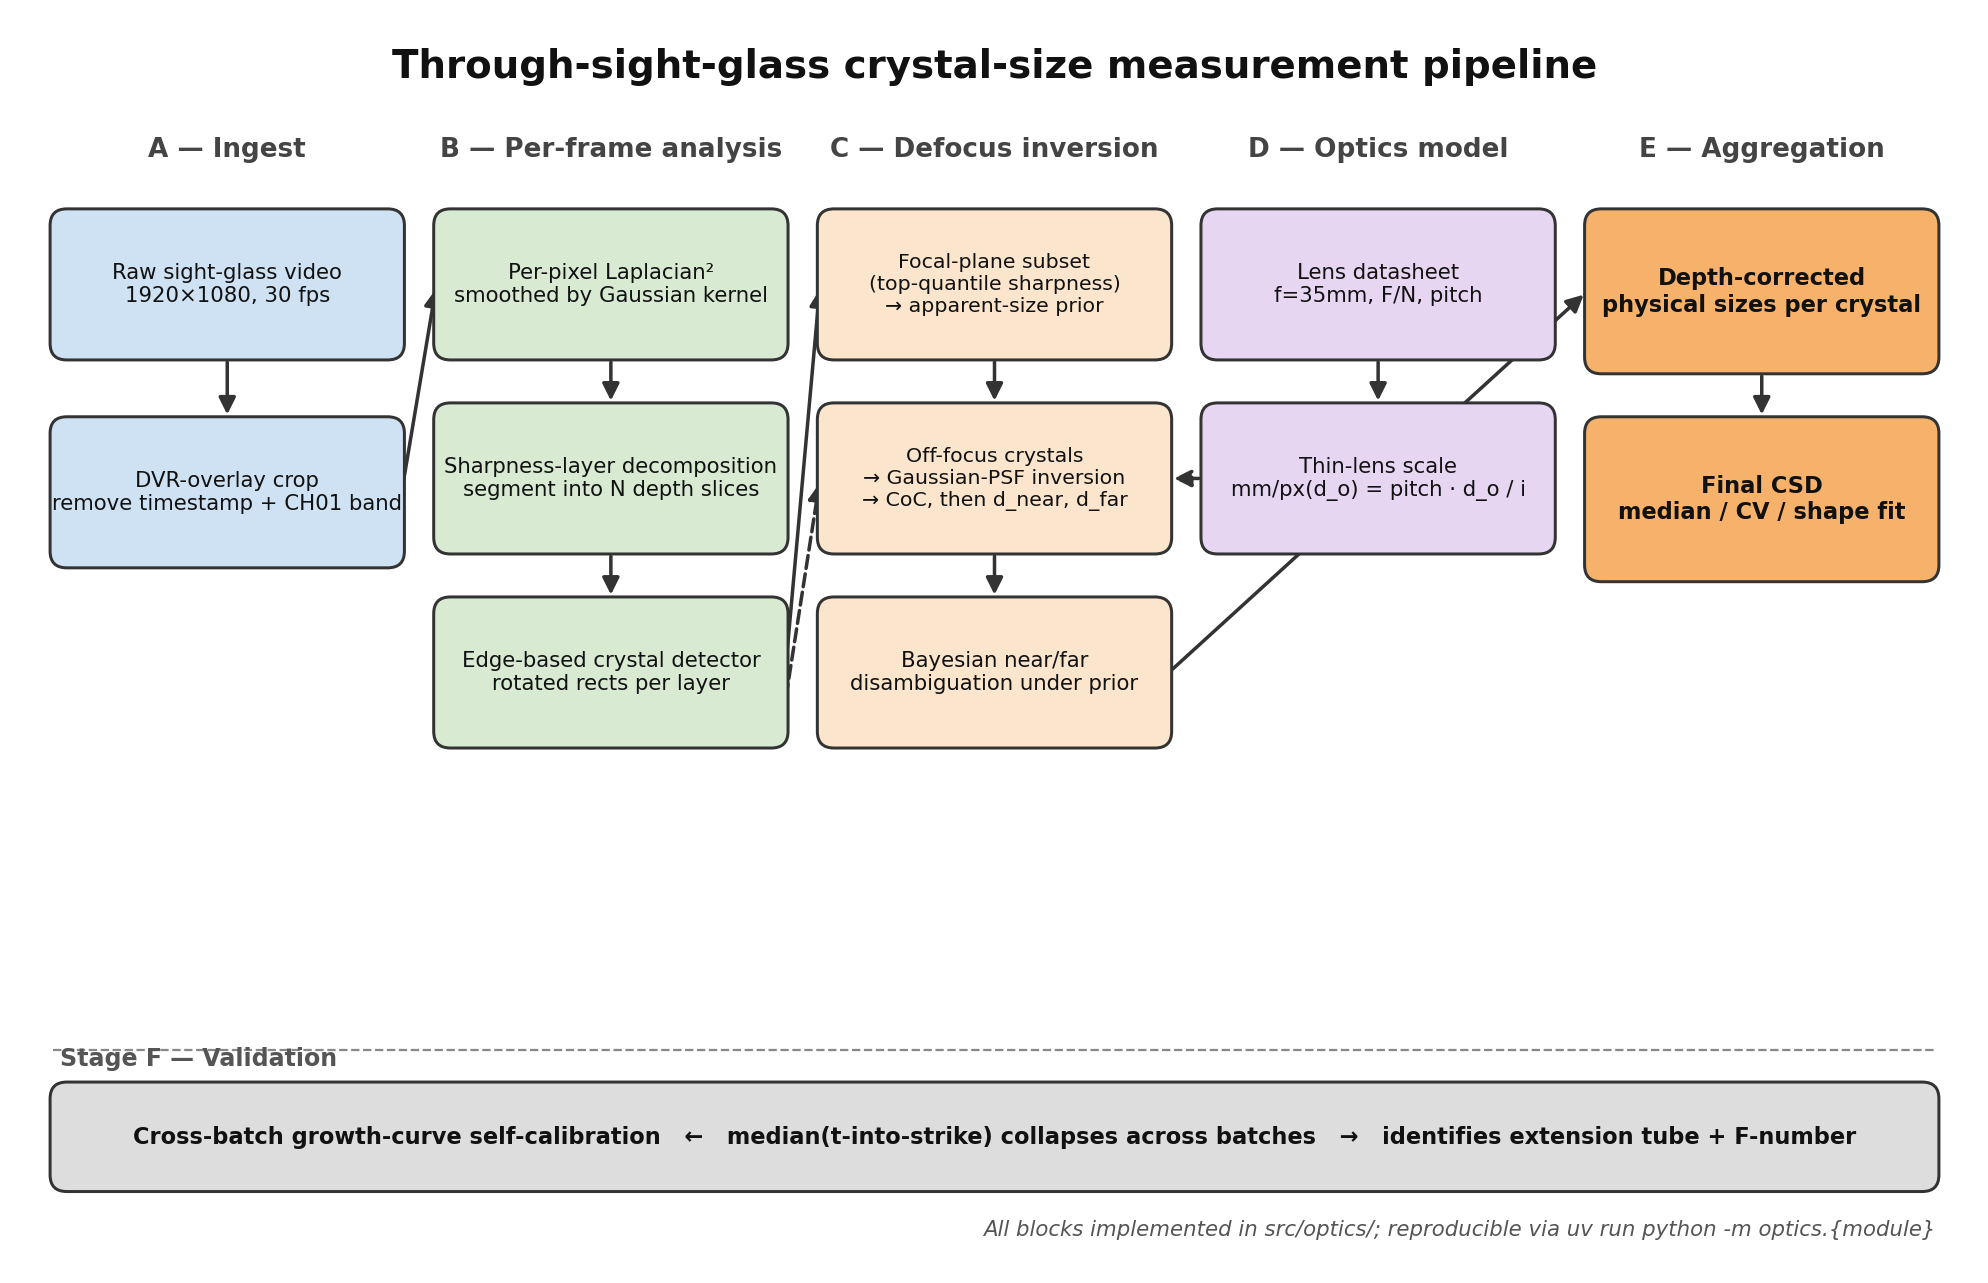
\includegraphics[width=0.75\textwidth]{13_pipeline}
\caption{\textbf{What is the full pipeline, end to end?} Stages A--E (top row) compose the forward measurement: raw
video $\rightarrow$ DVR-overlay crop $\rightarrow$ per-frame sharpness analysis $\rightarrow$ per-crystal defocus
inversion $\rightarrow$ thin-lens optics scale $\rightarrow$ aggregated CSD. Stage F (bottom bar) is the cross-batch
growth-curve self-validation discussed in \secref{sec:growth}. Every block is implemented as a reproducible Python
module under \texttt{src/optics/} and is exercised by the case-study run of
\S\S\,\ref{sec:optics}--\ref{sec:csd}.}\label{fig:pipeline}
\end{figure*}

\subsection{Contributions}\label{sec:contrib}

\begin{enumerate}
\item \textbf{A complete, open-source pipeline} that delivers calibrated CSD from raw through-sight-glass video by
integrating geometric optics, defocus analysis, Bayesian disambiguation, and growth-curve self-validation. MIT
licence, code at \emph{(URL)}.
\item \textbf{A single-component depth-aware sizing framework} that breaks the front/back defocus ambiguity using the
focal-plane apparent-size distribution as prior, under a documented homogeneous-slurry assumption that admits a
built-in self-consistency check (\secref{sec:sizing}).
\item \textbf{A quantitative treatment of detector--depth interaction}, including the explicit conditions under which
the disambiguation regime is operationally resolvable and the discriminability ceiling imposed by edge-based
detectors (\secref{sec:selectivity}).
\item \textbf{A validated industrial case study} at Slovensk\'e cukrovary, Sere\v{d}, demonstrating the pipeline on
archived video with a complete numerical audit trail.
\item \textbf{An honest failure-mode discussion} including the DVR-overlay contamination we encountered, the loss of
disambiguation power when the detector's depth selectivity is too narrow, and the refractive limits of the paraxial
sight-glass model.
\end{enumerate}
